
%================================
\subsection{Resultados de la implementación con OpenMP}
\label{sec:Resultados de la implementación con OpenMP}

\begin{table}[H]
   \centering
   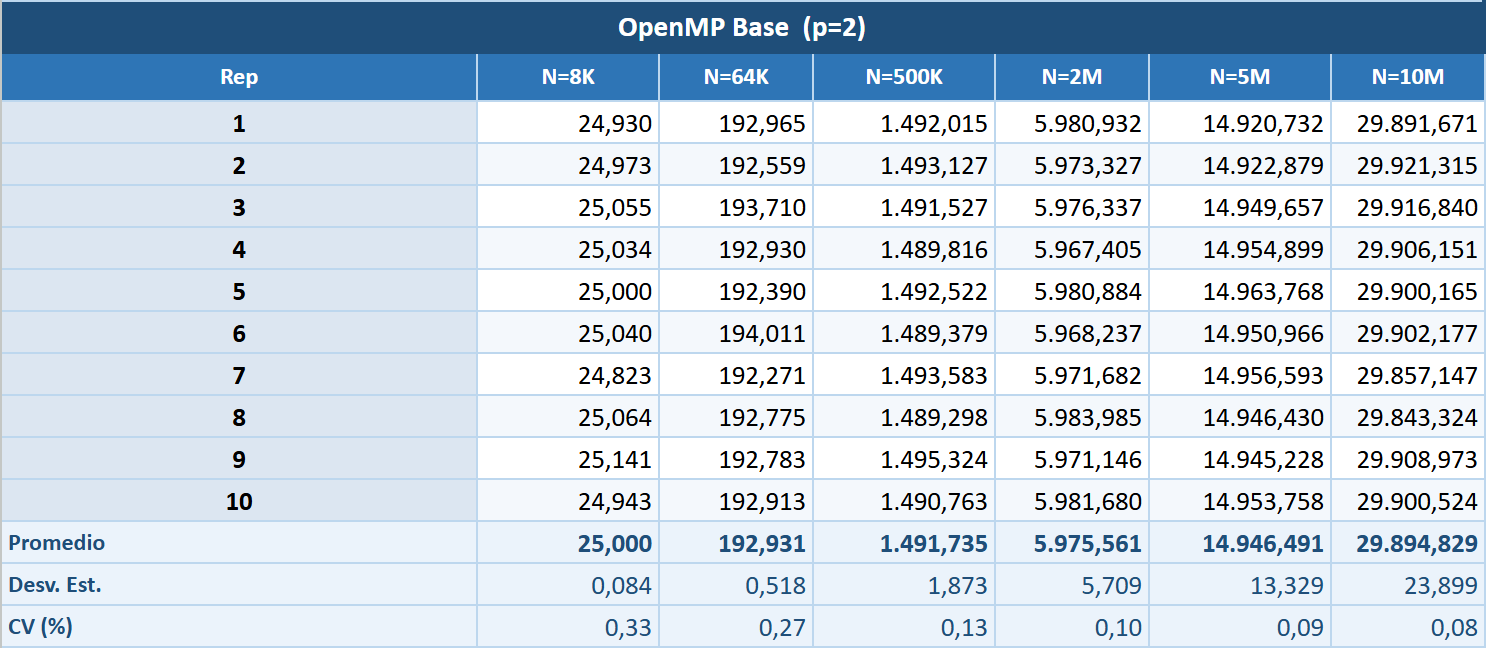
\includegraphics[width=1\textwidth]{images/results/tables/time_omp_2.png}
   \caption{Tiempos de ejecución del algoritmo paralelo con OpenMP utilizando 2 hilos}
\end{table}

\begin{table}[H]
   \centering
   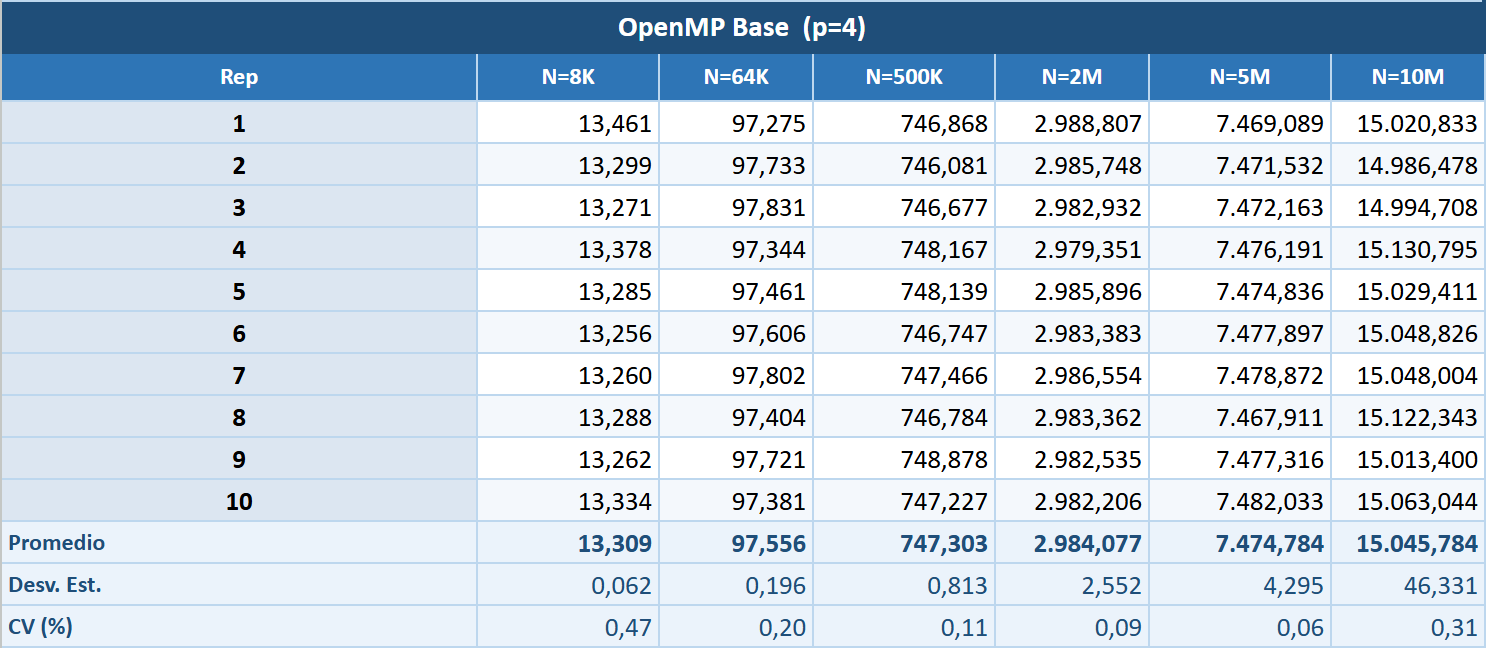
\includegraphics[width=1\textwidth]{images/results/tables/time_omp_4.png}
   \caption{Tiempos de ejecución del algoritmo paralelo con OpenMP utilizando 4 hilos}
\end{table}

\begin{table}[H]
   \centering
   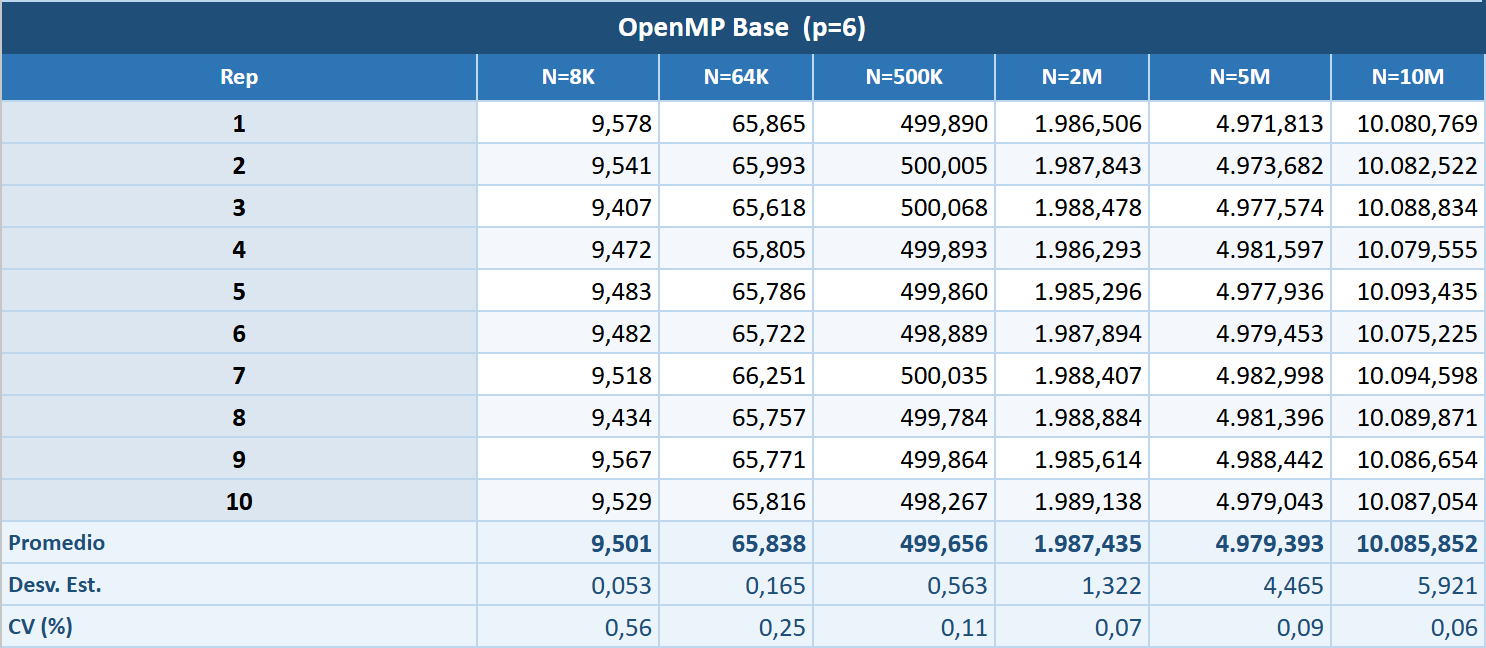
\includegraphics[width=1\textwidth]{images/results/tables/time_omp_6.png}
   \caption{Tiempos de ejecución del algoritmo paralelo con OpenMP utilizando 6 hilos}
\end{table}

\begin{table}[H]
   \centering
   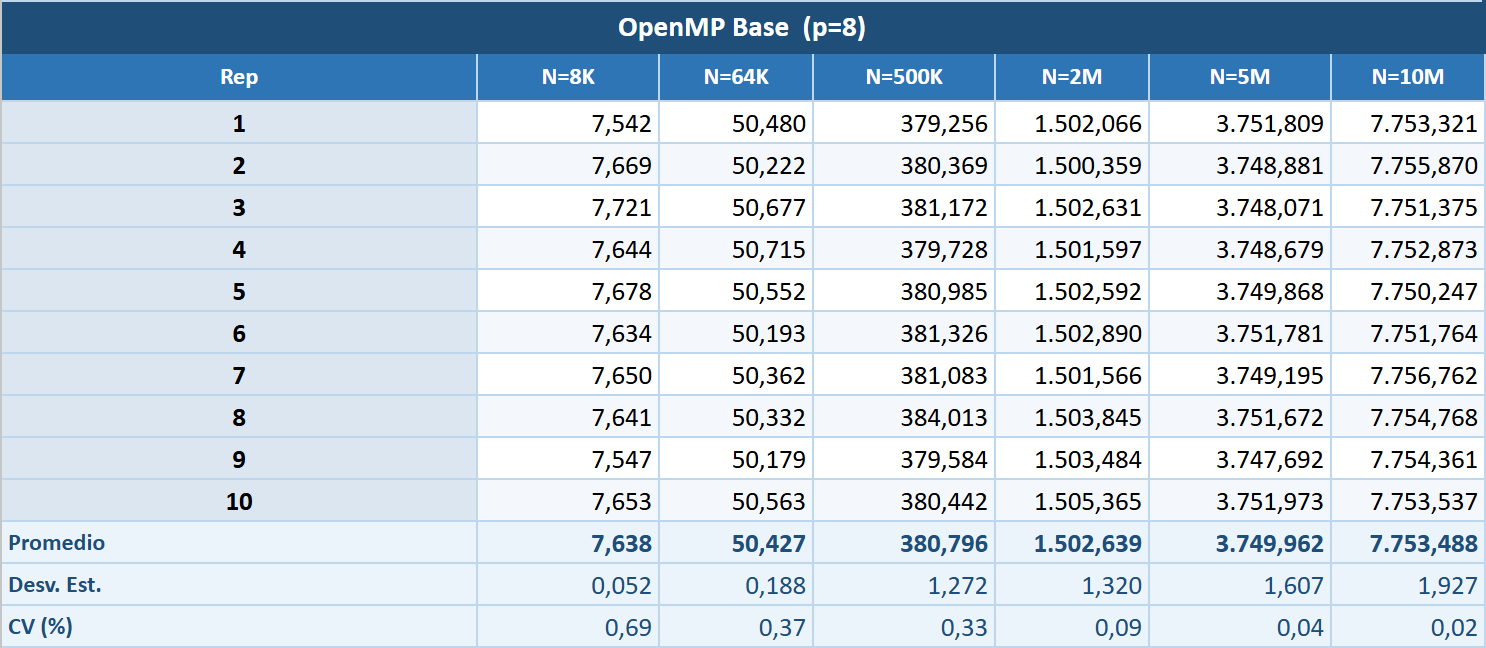
\includegraphics[width=1\textwidth]{images/results/tables/time_omp_8.png}
   \caption{Tiempos de ejecución del algoritmo paralelo con OpenMP utilizando 8 hilos}
\end{table}

\begin{table}[H]
   \centering
   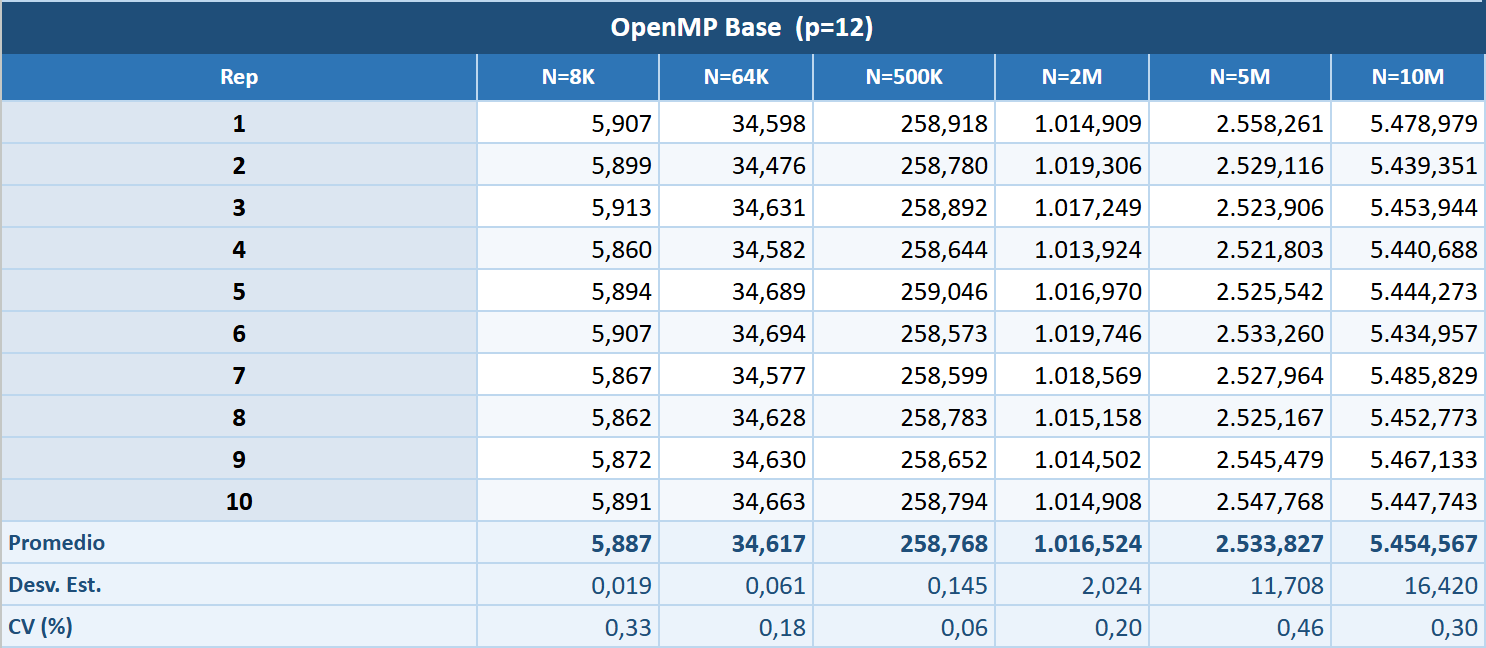
\includegraphics[width=1\textwidth]{images/results/tables/time_omp_12.png}
   \caption{Tiempos de ejecución del algoritmo paralelo con OpenMP utilizando 12 hilos}
\end{table}

\begin{table}[H]
   \centering
   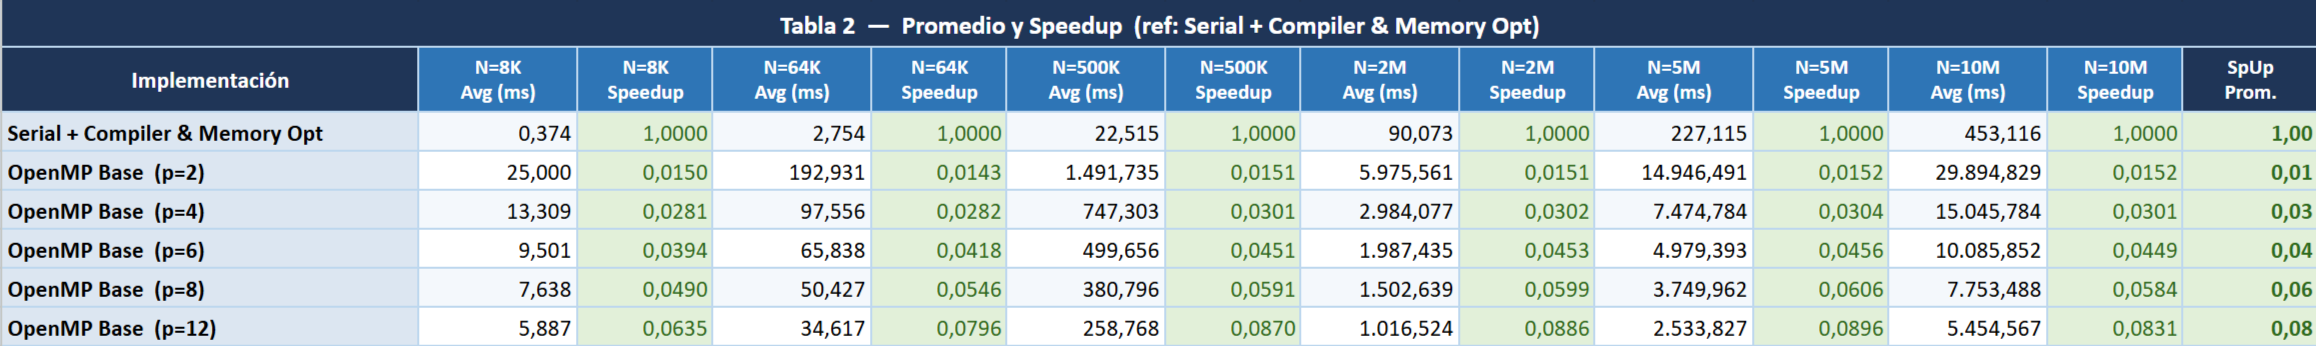
\includegraphics[width=1\textwidth]{images/results/tables/speedup_omp.png}
   \caption{Speedup del algoritmo paralelo con OpenMP}
\end{table}

\begin{figure}[H]
   \centering
   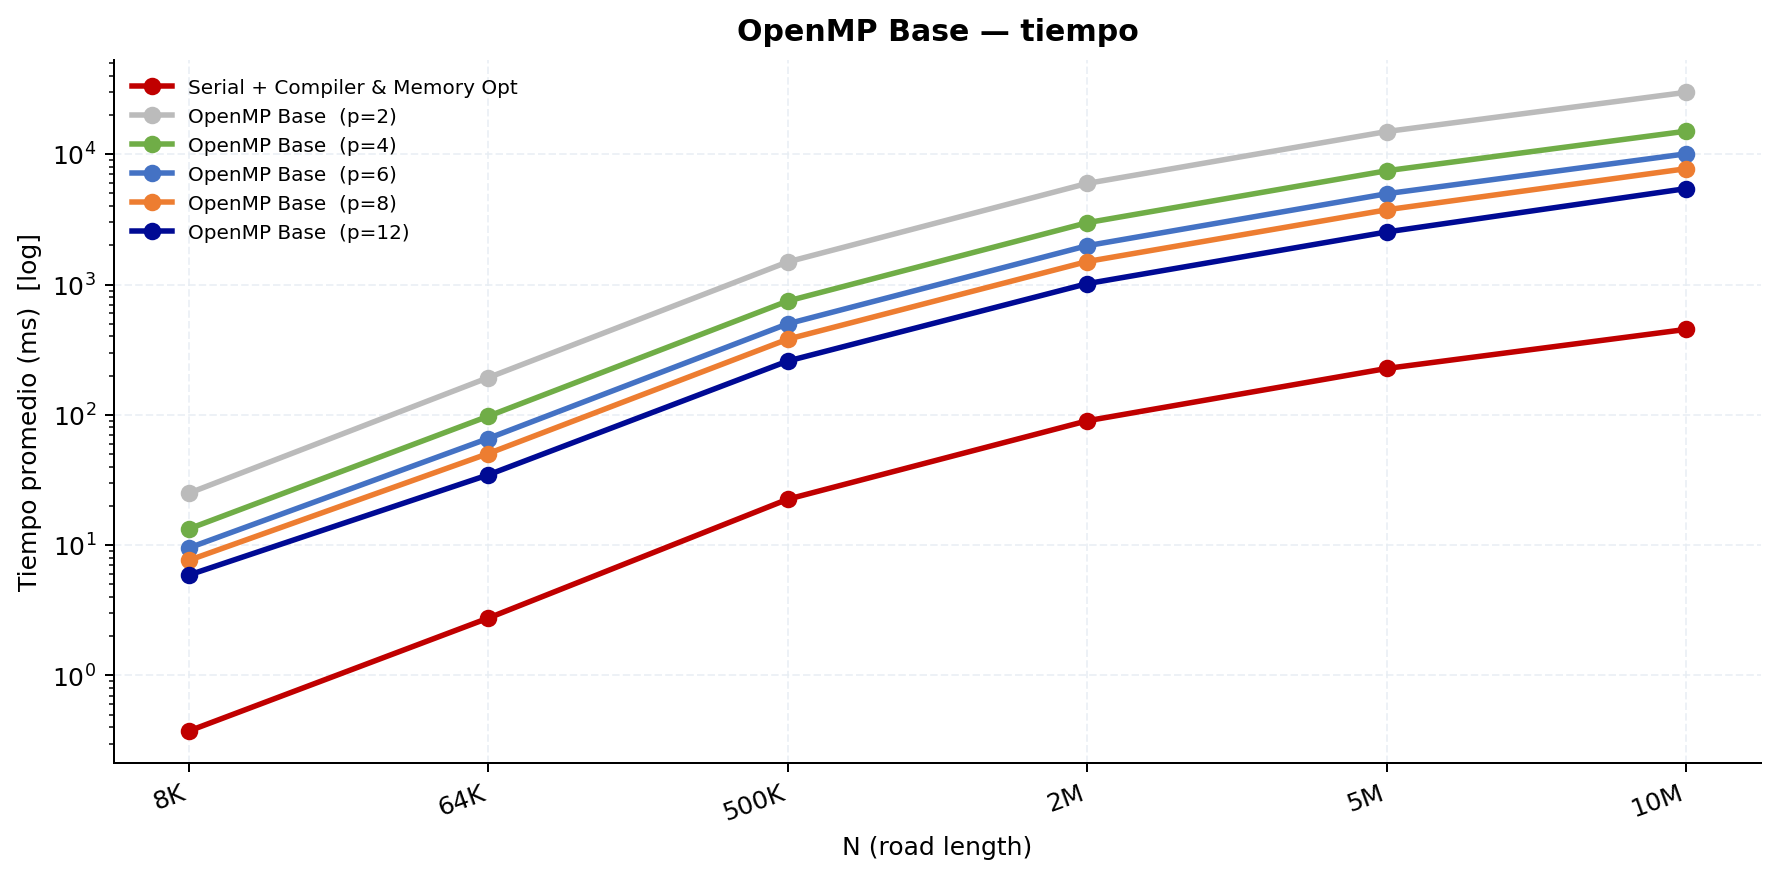
\includegraphics[width=1\textwidth]{images/results/charts/fig_omp_base_time.png}
   \caption{Tiempos de ejecución del algoritmo paralelo con OpenMP}
\end{figure}

\begin{figure}[H]
   \centering
   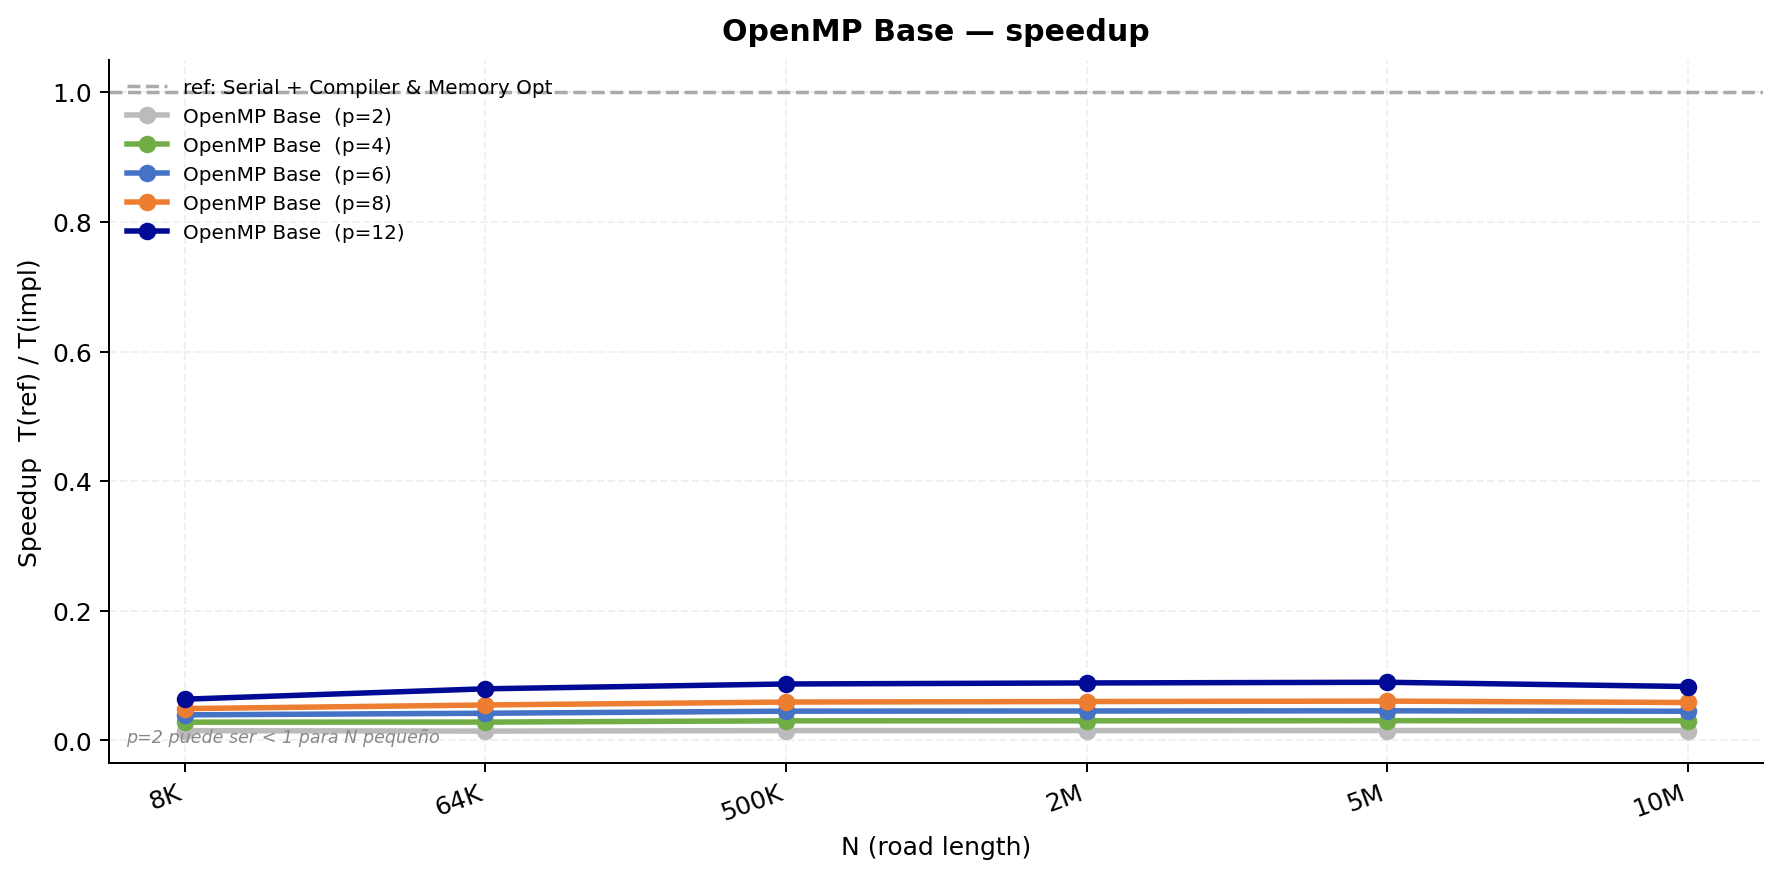
\includegraphics[width=1\textwidth]{images/results/charts/fig_omp_base_speedup.png}
   \caption{Speedup del algoritmo paralelo con OpenMP}
\end{figure}